\documentclass[a4paper,10pt]{article}
\usepackage[brazilian]{babel}
\usepackage[left=2.5cm,right=2.5cm,top=3cm,bottom=2.5cm]{geometry}
\usepackage{mathtools}
\usepackage{amsthm}
\usepackage{amsmath}
%\usepackage{nccmath}
\usepackage{amssymb}
\usepackage{amsfonts}
\usepackage{physics}
%\usepackage{dsfont}
%\usepackage{mathrsfs}

\usepackage{titling}
\usepackage{indentfirst}

\usepackage{bm}
\usepackage[dvipsnames]{xcolor}
\usepackage{cancel}

\usepackage{xurl}
\usepackage[colorlinks=true]{hyperref}

\usepackage{float}
\usepackage{graphicx}
%\usepackage{tikz}
\usepackage{caption}
\usepackage{subcaption}

%%%%%%%%%%%%%%%%%%%%%%%%%%%%%%%%%%%%%%%%%%%%%%%%%%%

\newcommand{\eps}{\epsilon}
\newcommand{\vphi}{\varphi}
\newcommand{\cte}{\text{cte}}

\newcommand{\N}{\mathbb{N}}
\newcommand{\Z}{\mathbb{Z}}
\newcommand{\Q}{\mathbb{Q}}
\newcommand{\R}{\vb{R}}
\newcommand{\C}{\mathbb{C}}
\renewcommand{\S}{\hat{S}}
%\renewcommand{\H}{\s{H}}

\renewcommand{\a}{\vb{a}}
\newcommand{\nn}{\hat{n}}
\renewcommand{\d}{\dagger}
\newcommand{\up}{\uparrow}
\newcommand{\down}{\downarrow}

\newcommand{\0}{\vb{0}}
%\newcommand{\1}{\mathds{1}}
\newcommand{\E}{\vb{E}}
\newcommand{\B}{\vb{B}}
\renewcommand{\v}{\vb{v}}
\renewcommand{\r}{\vb{r}}
\renewcommand{\k}{\vb{k}}
\newcommand{\p}{\vb{p}}
\newcommand{\q}{\vb{q}}
\newcommand{\F}{\vb{F}}

\newcommand{\s}{\sigma}
%\newcommand{\prodint}[2]{\left\langle #1 , #2 \right\rangle}
\newcommand{\cc}[1]{\overline{#1}}
\newcommand{\Eval}[3]{\eval{\left( #1 \right)}_{#2}^{#3}}

\newcommand{\unit}[1]{\; \mathrm{#1}}

\newcommand{\n}{\medskip}
\newcommand{\e}{\quad \mathrm{e} \quad}
\newcommand{\ou}{\quad \mathrm{ou} \quad}
\newcommand{\virg}{\, , \;}
\newcommand{\ptodo}{\forall \,}
\renewcommand{\implies}{\; \Rightarrow \;}
%\newcommand{\eqname}[1]{\tag*{#1}} % Tag equation with name

\setlength{\droptitle}{-7em}

\theoremstyle{plain}
\newtheorem{theorem}{Teorema}[section]
%\newtheorem{defi}[theorem]{Definição}
\newtheorem{lemma}[theorem]{Lema}
%\newtheorem{corol}[theorem]{Corolário}
%\newtheorem{prop}[theorem]{Proposição}
%\newtheorem{example}{Exemplo}
%
%\newtheorem{inneraxiom}{Axioma}
%\newenvironment{axioma}[1]
%  {\renewcommand\theinneraxiom{#1}\inneraxiom}
%  {\endinneraxiom}
%
%\newtheorem{innerpostulado}{Postulado}
%\newenvironment{postulado}[1]
%  {\renewcommand\theinnerpostulado{#1}\innerpostulado}
%  {\endinnerpostulado}
%
%\newtheorem{innerexercise}{Exercício}
%\newenvironment{exercise}[1]
%  {\renewcommand\theinnerexercise{#1}\innerexercise}
%  {\endinnerexercise}
%
%\newtheorem{innerthm}{Teorema}
%\newenvironment{teorema}[1]
%  {\renewcommand\theinnerthm{#1}\innerthm}
%  {\endinnerthm}
%
\newtheorem{innerlema}{Lema}
\newenvironment{lema}[1]
  {\renewcommand\theinnerlema{#1}\innerlema}
  {\endinnerlema}
%
%\theoremstyle{remark}
%\newtheorem*{hint}{Dica}
%\newtheorem*{notation}{Notação}
%\newtheorem*{obs}{Observação}


\title{\Huge{\textbf{Lista 2 - Mecânica Estatística}}}
\author{Mateus Marques}

\begin{document}

\maketitle

\section*{2) Oscilador harmônico no ensemble canônico}

(a) Para contar todos os microestados com energia variável no cálculo da função de partição, integramos todas as variáveis $q_i, p_i$ sobre todos os valores possíveis:
$$
Z_N = \int_{-\infty}^{\infty}\int_{-\infty}^{\infty} \frac{\dd{p_1} \dd{q_1}}{2\pi\hbar} \cdots \int_{-\infty}^{\infty}\int_{-\infty}^{\infty} \frac{\dd{p_N} \dd{q_N}}{2\pi\hbar} e^{-\beta H(\q, \p)} =
$$
$$
= \qty{\frac{1}{2\pi\hbar} \int_{-\infty}^{\infty} e^{-\beta \frac{p^2}{2m}} \dd{p} \int_{-\infty}^{\infty} e^{-\beta \frac{m\omega^2q^2}{2} }\dd{q}}^N =
\qty[ \frac{1}{2\pi\hbar} \sqrt{\frac{2m\pi}{\beta}} \sqrt{\frac{2\pi}{m\omega^2\beta}} ]^N =
\qty(\frac{1}{\beta \hbar \omega})^N = \qty(\frac{k_B T}{\hbar \omega})^N.
$$

\begin{itemize}
\item A energia livre é dada por
$$
F = - k_B T \log Z = -\frac{1}{\beta} N \log(\frac{1}{\beta \hbar \omega}) = \frac{N}{\beta} \log(\beta\hbar\omega) =
-N k_B T \log(\frac{k_B T}{\hbar \omega}).
$$

\item A energia interna é
$$
E = \frac{\tr(H e^{-\beta H})}{\tr(e^{-\beta H})} = - \frac{1}{Z} \pdv{Z}{\beta} = - \pdv{\log Z}{\beta} =
N\pdv{\log(\beta\hbar\omega)}{\beta} = \frac{N}{\beta} = N k_B T,
$$
que corresponde ao que obtemos na lista 1 para o ensemble microcanônico.

\item Da definição termodinâmica de energia livre $F = E - TS$, temos que a entropia é
$$
S = \frac{E-F}{T} = \frac{N k_B T + N k_B T \log(\frac{k_B T}{\hbar\omega})}{T} = N k_B \qty[1 + \log(\frac{k_B T}{\hbar\omega})],
$$
que também é a mesma entropia obtida na lista 1.

\item Pressão:
$$
P = -\pdvc{F}{V}{T,N} = 0,
$$
porque o sistema não depende do volume, como foi discutido na lista 1.

\item Potencial químico:
$$
\mu = \pdvc{F}{N}{T,V} = - k_B T \log(\frac{k_B T}{\hbar\omega}),
$$
que também está de acordo com o que obtivemos no ensemble microcanônico.
\end{itemize}

(b) A função de partição no caso quântico é
$$
Z_N = \sum_{n_1 = 0}^{\infty} \sum_{n_2 = 0}^{\infty} \cdots \sum_{n_N = 0}^{\infty} e^{-\beta \sum_{j=1}^{N} E_n^j} =
\qty(\sum_{n=0}^{\infty} e^{-\beta E_n})^N =
$$
$$
= \qty(e^{-\beta \hbar \omega / 2} \sum_{n=0}^{\infty} e^{-\beta n \hbar\omega})^N =
\qty(\frac{e^{-\beta \hbar \omega / 2}}{1 - e^{-\beta\hbar\omega}})^N =
\qty[\frac{1}{2\sinh(\frac{\beta\hbar\omega}{2})}]^N.
$$

A energia livre é dada por
\begin{equation} \label{eq:free_energy-1qu}
F = - \frac{1}{\beta} \log Z = \frac{N}{\beta} \log\qty[2 \sinh(\frac{\beta\hbar\omega}{2})] =
N k_B T \log\qty[2 \sinh(\frac{\hbar\omega}{2 k_B T})].
\end{equation}

A entropia pode ser calculada por
$$
S = -\pdvc{F}{T}{V,N} = - N k_B \log\qty[2 \sinh(\frac{\hbar\omega}{2 k_B T})] -
N k_B T \frac{2 \cosh(\frac{\hbar\omega}{2 k_B T})}{2 \sinh(\frac{\hbar\omega}{2 k_B T})} \,
\qty(-\frac{\hbar\omega}{2 k_B T^2}) \implies
$$
$$
\boxed{
S = - N k_B \log\qty[2 \sinh(\frac{\hbar\omega}{2 k_B T})] + \frac{N\hbar\omega}{2 T} \coth(\frac{\hbar\omega}{2 k_B T}).
}
$$
Notando que na expressão acima a fórmula \ref{eq:free_energy-1qu} da energia livre reaparece no primeiro termo, temos que
$$
S = - \frac{F}{T} + \frac{N\hbar\omega}{2 T} \coth(\frac{\hbar\omega}{2 k_B T}) \implies
\boxed{ E = T \qty(S + \frac{F}{T}) = \frac{N\hbar\omega}{2} \coth(\frac{\hbar\omega}{2 k_B T}). }
$$

O calor específico $C_V$ é então
$$
C_V = \pdvc{E}{T}{V,N} =
- \frac{N\hbar\omega}{2} \frac{1}{\sinh[2](\frac{\hbar\omega}{2 k_B T})} \qty(-\frac{\hbar\omega}{2 k_B T^2}) \implies
\boxed{
C_V =
\frac{N (\hbar\omega)^2}{4 k_B T^2} \cdot \frac{1}{\sinh[2](\frac{\hbar\omega}{2 k_B T})}.
}
$$

\n

Como $\hat{H} = \sum_{i} \hbar\omega(\hat{N}_i + \frac{1}{2})$, temos que a ocupação média $\ev{n} = \frac{1}{N} \sum_{i} \ev{\hat{N}_i}$ satisfaz
$$
E = \ev{\hat{H}} = N \hbar\omega\qty(\ev{n} + \frac{1}{2}),
$$
portanto
$$
\ev{n} = \frac{1}{2} \qty[\coth(\frac{\hbar\omega}{2 k_B T}) - 1].
$$
Reescrevendo $\coth x - 1 = \frac{e^x + e^{-x}}{e^x - e^{-x}} - 1 = \frac{e^{2x} + 1}{e^{2x} - 1} - \frac{e^{2x} - 1}{e^{2x} - 1} = \frac{2}{e^{2x} - 1}$, temos
$$
\boxed{ \ev{n} = \frac{1}{e^{\frac{\hbar\omega}{k_B T}} - 1}, }
$$
que é a distribuição de Bose-Einstein.

\n

\begin{figure}[H]
\centering
\begin{subfigure}{.46\textwidth}
  \centering
  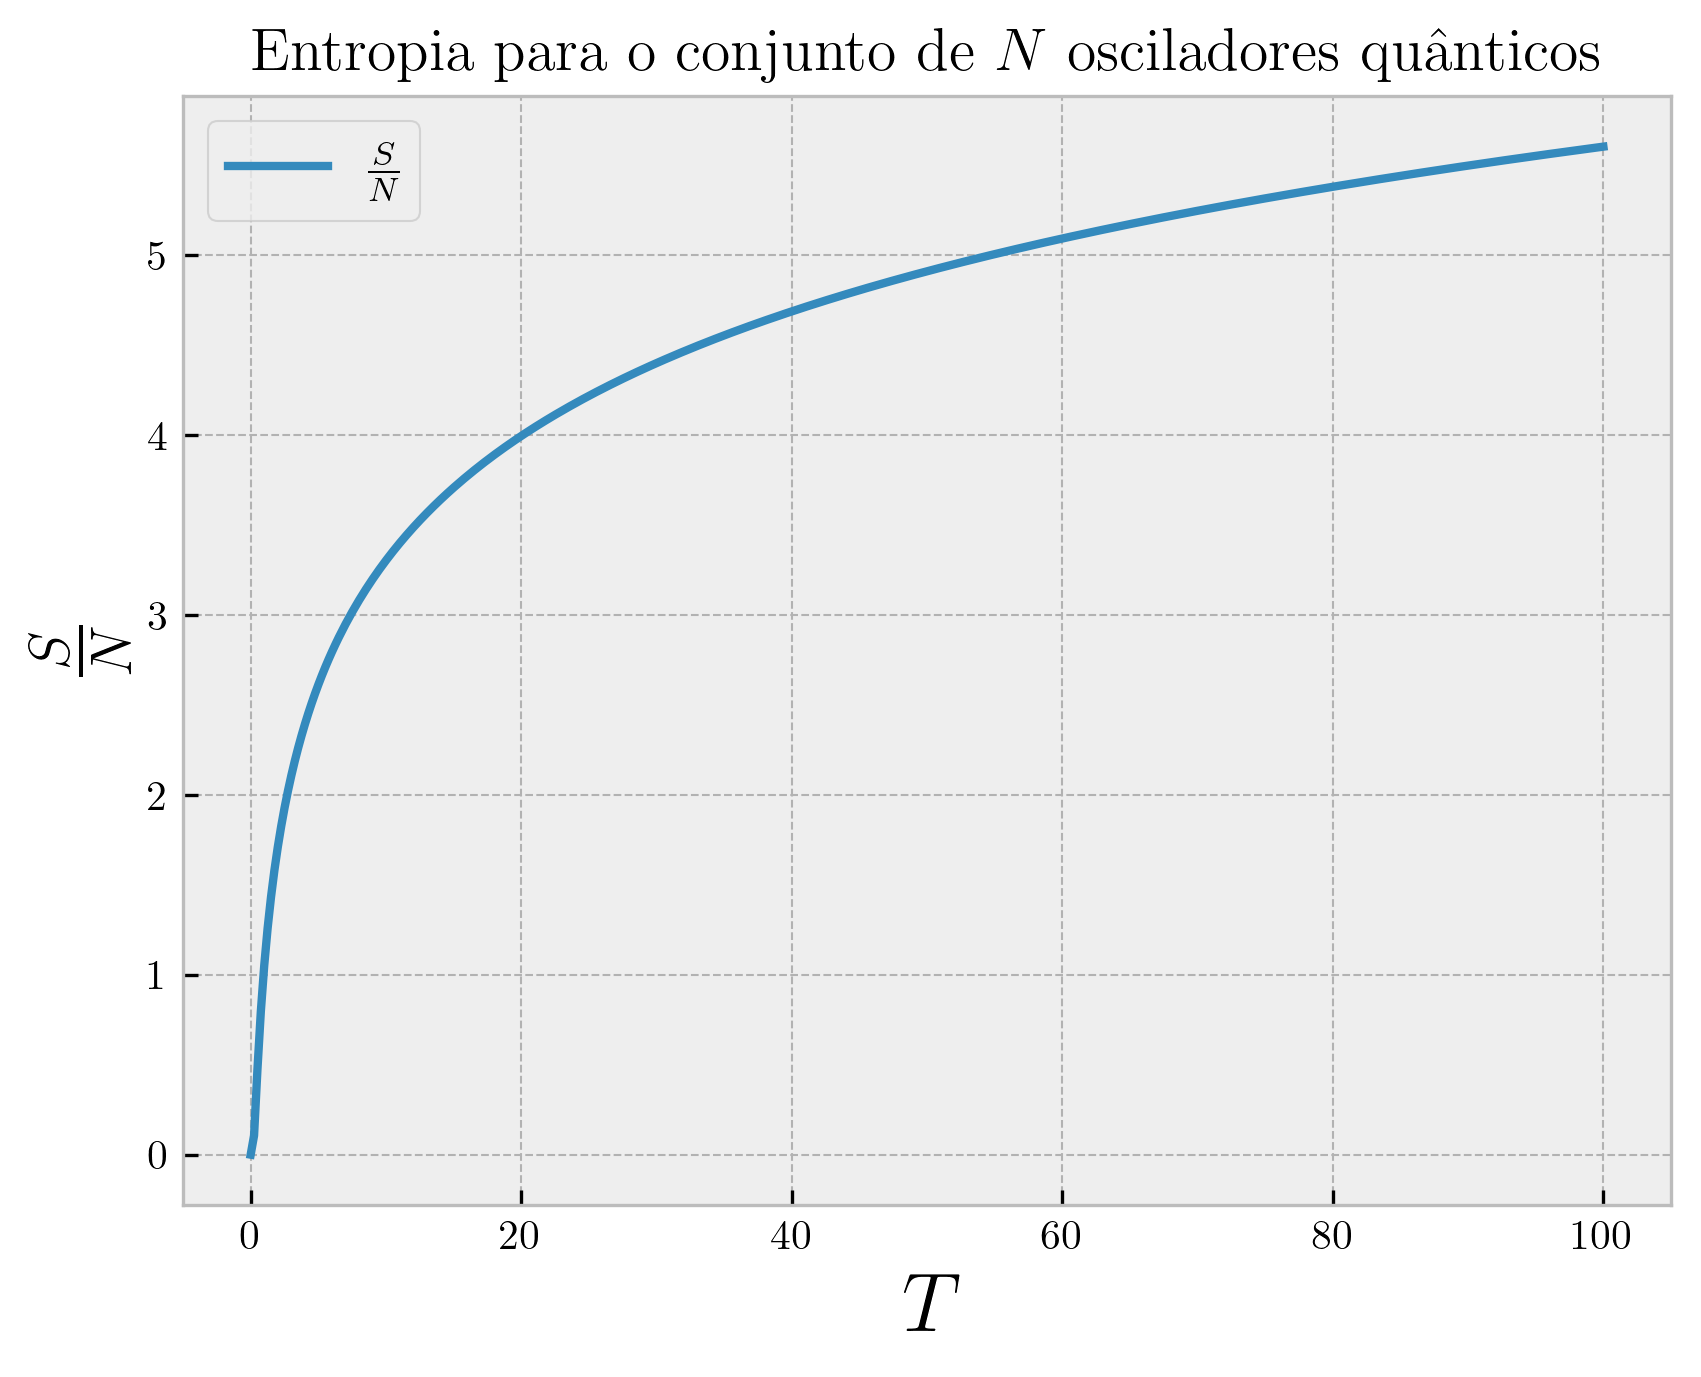
\includegraphics[width=0.95\linewidth]{fig/entropia_quant-osc.png}
  \label{fig:entropia_qosc}
\end{subfigure}
\begin{subfigure}{.46\textwidth}
  \centering
  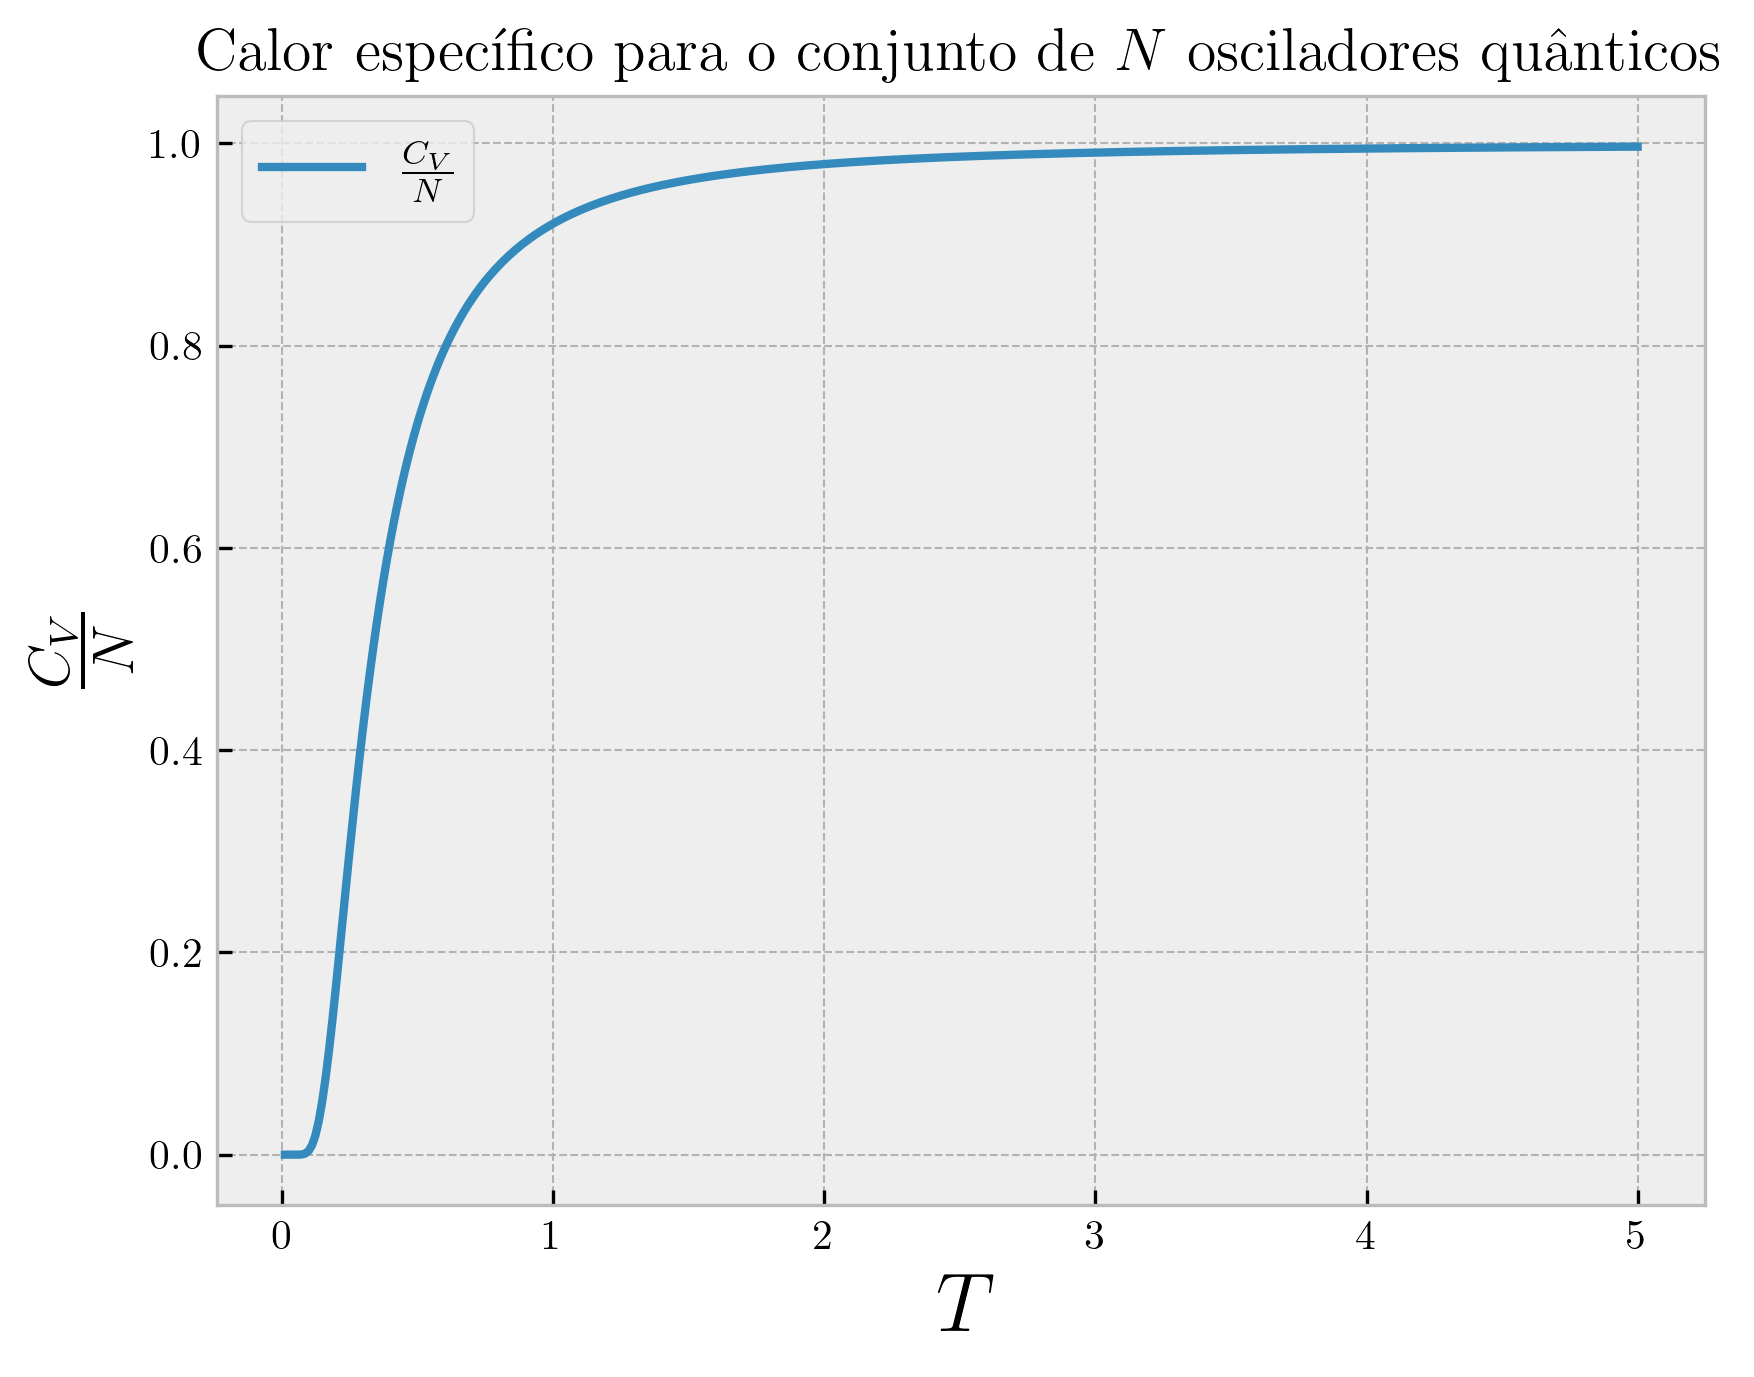
\includegraphics[width=0.95\linewidth]{fig/cv_quant-osc.png}
  \label{fig:cv_qosc}
\end{subfigure}
\label{fig:qosc}
\caption{Lado esquerdo curva $S/N \times T$ e lado direito curva $C_V/N \times T$. Em ambas as figuras utilizei as unidades arbitrárias $\hbar = \omega = k_B = 1$.}
\end{figure}

No limite $T \to 0$ temos que tanto $S$ como $C_V$ tendem a zero. Para $T \to \infty$, $\sinh(\frac{\hbar\omega}{2k_B T}) \approx \frac{\hbar\omega}{2k_B T}$, de maneira que
$$
\lim_{T\to\infty} C_V(T) = N k_B,
$$
o que condiz com o resultado clássico do gás ideal. Para a entropia, no limite $T \to \infty$ temos
$$
S = - N k_B \log\qty[2 \sinh(\frac{\hbar\omega}{2 k_B T})] + \frac{N\hbar\omega}{2 T} \coth(\frac{\hbar\omega}{2 k_B T})
\approx
$$
$$
- N k_B \log\qty[2 \frac{\hbar\omega}{2 k_B T}] +
\frac{N\hbar\omega}{2 T}\cdot\frac{2 k_B T}{\hbar\omega} =
- N k_B \log\qty(\frac{\hbar\omega}{k_B T}) + N k_B \implies
$$
$$
S \approx
N k_B \qty[1 + \log\qty(\frac{k_B T}{\hbar\omega})],
$$
que é justamente o resultado clássico obtido no item (a). Vemos então que recuperamos o limite clássico quando $T \to \infty$, ou equivalentemente quando $\hbar \to 0$, o que faz muito sentido.



\pagebreak

\section*{4) Distribuição de Maxwell}

(a) Sendo $p(\v)$ a probabilidade de encontrar uma partícula no volume $\dd[3]{\v}$, como $\v = \p/m$, temos que $p(\v) \dd[3]{\v}$ equivale à probabilidade de encontrar a partícula com momento no elemento $\dd[3]{\p}$ e no volume $V$. Como $E = \p^2/2m$, do ensemble canônico temos
$$
p(\v) \dd[3]{\v} = \frac{V}{Z_1} \exp(- \frac{\beta \p^2}{2m}) \dd[3]{\p} = \frac{V}{m^3 Z_1} \exp(- \frac{\beta m \v^2}{2}) \dd[3]{\v},
$$
onde
$$
Z_1 = \int \dd[3]{\r} \int \dd[3]{\p} \, \exp(\frac{-\beta \p^2}{2m}) = V \qty(\frac{2\pi m}{\beta})^{3/2}.
$$

Concluimos então que
$$
\boxed{ p(\v) = \exp(-\frac{m \v^2}{2 k_B T}) \qty(\frac{2\pi k_B T}{m})^{-3/2}. }
$$

Para obter a distribuição do módulo de velocidades, basta notar que a densidade de probabilidade $p(v)$ não depende da direção de $\v$, somente de seu módulo $v$. Assim, integrando sobre o ângulo sólido $\int \dd{\Omega} = \int \dd{\cos\theta} \int \dd{\vphi} = 4\pi$, temos
$$
f(v) \dd{v} = \int \dd{\Omega} \Big[ p(v) v^2 \dd{v} \Big] = 4\pi v^2 p(v) \dd{v},
$$
da onde tiramos que
$$
\boxed{ f(v) = 4 \pi v^2 p(v) = 4 \pi v^2 \exp(-\frac{m v^2}{2 k_B T}) \qty(\frac{2\pi k_B T}{m})^{-3/2}. }
$$

\begin{figure}[H]
\centering
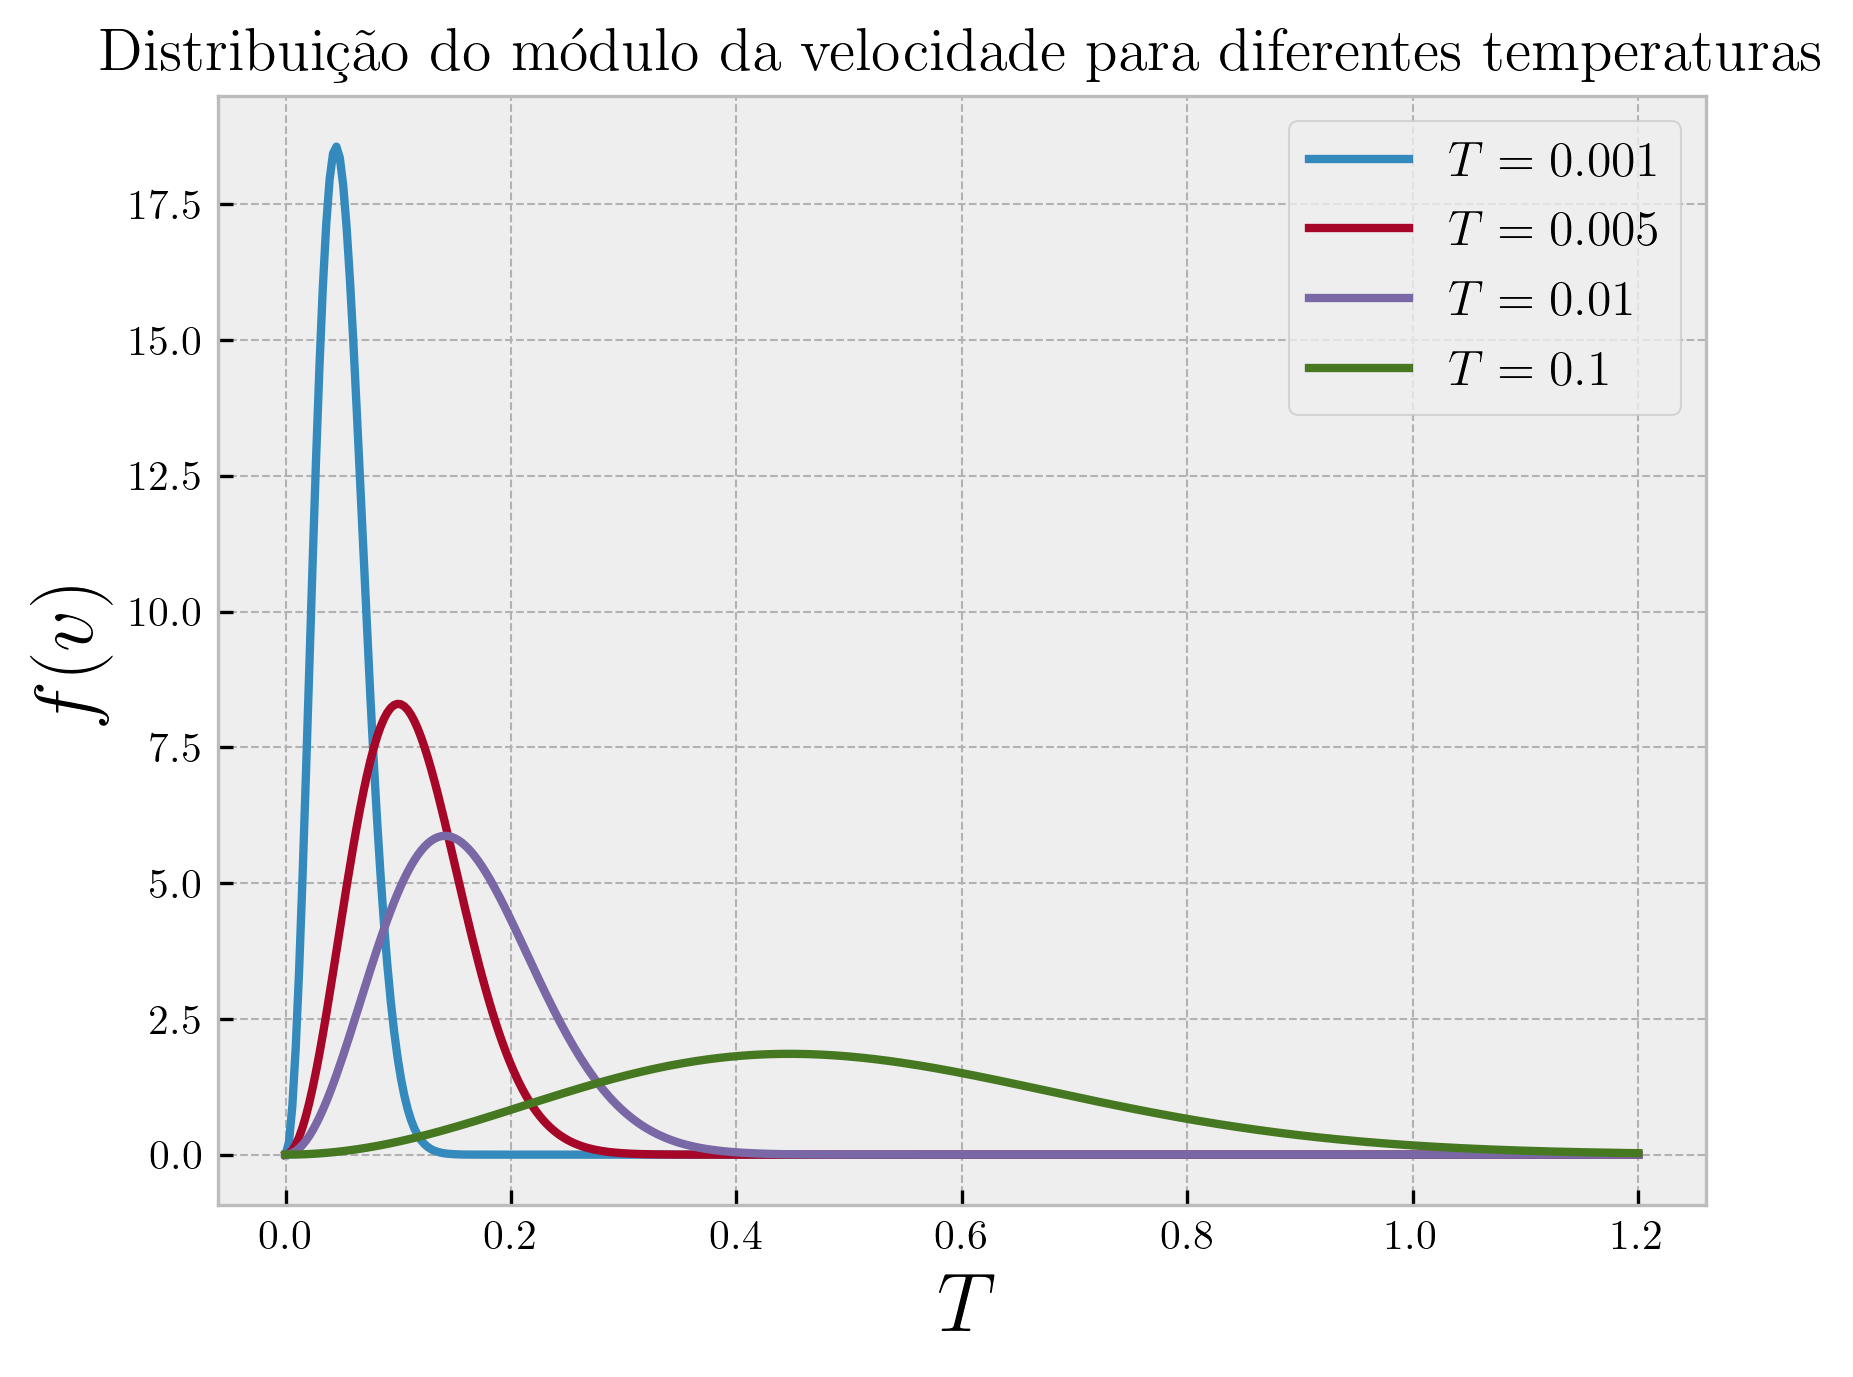
\includegraphics[width=0.7\linewidth]{fig/distrib-vel-maxwell.png}
\caption{Distribuição de Maxwell para as velocidades em diferentes temperaturas. Utilizei unidades arbitrárias em que $k_B = m = 1$.}
\label{fig:maxwell}
\end{figure}

(b) Temos que
$$
\ev{v^2} = \int_0^\infty v^2 f(v) \dd{v} = 4\pi \qty(\frac{2\pi k_B T}{m})^{-3/2}
\int_0^\infty v^4 \exp(-\frac{\beta m v^2}{2}) \dd{v}.
$$
Fazendo a substituição $u = \frac{\beta m v^2}{2}$, temos que $\dd{u} = \beta m v \dd{v}$ e a integral acima fica
$$
\int_0^\infty v^4 \exp(-\frac{\beta m v^2}{2}) \dd{v} =
\int_0^\infty \qty(\frac{2u}{\beta m})^{3/2} e^{-u} \frac{\dd{u}}{\beta m} =
$$
$$
= \frac{1}{\beta m} \qty(\frac{2}{\beta m})^{3/2} \int_0^\infty u^{5/2 - 1} e^{-u} \dd{u}.
$$
A integral acima é o valor particular $z = 5/2$ da função gamma $\Gamma(z) = \int_0^\infty t^{z-1} e^{-t} \dd{t}$ (\url{https://en.wikipedia.org/wiki/Gamma_function}), onde o Mathematica retorna $\Gamma(5/2) = \frac{3}{4} \sqrt{\pi}$. Portanto
$$
\ev{v^2} = 4\pi \qty(\frac{2\pi}{\beta m})^{-3/2} \frac{1}{\beta m} \qty(\frac{2}{\beta m})^{3/2} \frac{3}{4} \sqrt{\pi} =
\frac{3}{\beta m} \implies
\boxed{ \sqrt{\ev{v^2}} = \sqrt{\frac{3k_B T}{m}}. }
$$

Agora, a localização do máximo de $f(v)$ é encontrada resolvendo $\dv{f}{v} = 0$. A derivada é
$$
\dv{f}{v} = 4\pi \qty(\frac{2\pi k_B T}{m})^{-3/2}
\qty[
2v - v^2 \beta m v
] \exp(-\beta m v^2/2).
$$
$$
\dv{f}{v} = 0 \implies 2v = v^3 \beta m \implies \boxed{ v_{\text{max}} = \sqrt{\frac{2 k_B T}{m}}. }
$$

Assim vemos que $v_{\text{max}} < \sqrt{\ev{v^2}}$, de maneira que $v_{\text{max}}/\sqrt{\ev{v^2}} = \sqrt{2/3} \approx 0.816$. Olhando para os gráficos da Figura \ref{fig:maxwell} vemos que esse resultado faz sentido. De fato, as distribuições são assimétricas. Os máximos são pontudos no começo e mais para frente a função decai, de maneira que essa contribuição para velocidades maiores faz com que $\sqrt{\ev{v^2}}$ seja maior que o ponto de máximo $v_{\text{max}}$.

\n

(c) Temos que
$$
\ev{\abs{\v_1 - \v_2}} = \int \dd[3]{\v_1} \int \dd[3]{\v_2} \abs{\v_1 - \v_2} \, p(\v_1) p(\v_2).
$$
Fazendo a substituição de variáveis $\u = \v_1 - \v_2$, $\v = \frac{\v_1 + \v_2}{2}$, que tem jacobiano unitário ($\dd[3]{\u} \dd[3]{\v} = \dd[3]{\v_1} \dd[3]{\v_2}$), temos que
$$
\ev{\abs{\v_1 - \v_2}} = \int \dd[3]{\u} \int \dd[3]{\v} \abs{\u} \, p(\v + \u/2) \, p(\v - \u/2) =
$$
$$
= \qty(\frac{2\pi}{\beta m})^{-3} \int \dd[3]{\u} \int \dd[3]{\v} \abs{\u}
\exp{-\frac{\beta m}{2} \qty[\qty(\v + \frac{\u}{2})^2 + \qty(\v - \frac{\u}{2})^2]} =
$$
$$
= \qty(\frac{2\pi}{\beta m})^{-3} \int \dd[3]{\u} \int \dd[3]{\v} \abs{\u}
\exp(-\beta m \v^2) \exp(-\frac{\beta m}{4} \u^2) =
$$
$$
= (4\pi)^2 \qty(\frac{2\pi}{\beta m})^{-3} \qty[ \int_0^\infty u^3 \exp(-\frac{\beta m}{4} u^2) \dd{u} ]
\qty[ \int_0^\infty v^2 \exp(-\beta m v^2) \dd{v} ] \implies
$$
$$
\boxed{\ev{\abs{\v_1 - \v_2}} = \frac{4}{\sqrt{\pi}} \, \sqrt{\frac{k_B T}{m}},}
$$
onde eu avaliei as últimas duas integrais em colchetes no Mathematica. Note que $4/\sqrt{\pi} \approx 2.257$. Dessa forma, temos que $\ev{\abs{\v_1 - \v_2}} > \sqrt{\ev{v^2}} > v_{\text{max}}$. Esse resultado faz sentido, pois o valor esperado $\ev{\abs{\v_1 - \v_2}}$ leva em conta as direções das velocidades $\v_1$ e $\v_2$. Mesmo que o módulo de $\v_1 = v$ seja igual a $\v_2 = v$, se elas apontarem em direções antiparalelas isso gera uma contribuição positiva de $2v$ para $\ev{\abs{\v_1 - \v_2}}$. Desse modo, é natural que essa quantidade seja maior que $\sqrt{\ev{v^2}}$ ou $v_{\text{max}}$.



\pagebreak

\section*{6) Magnetismo de gases}

(a) Tomando $\B = B \vu{k}$, a hamiltoniana do gás de momentos magnéticos clássico é
$$
E = - \sum_{i = 1}^{N} \mu B \cos\theta_i.
$$
Como já sabemos o comportamento de um gás ideal clássico (cada partícula livre com energia cinética $E = \p^2/2m$) e as energias livres se somam, focarei apenas nos graus de liberdade $(\theta_i, \vphi_i)$ que determinam a direção do momento magnético $\bm{\mu}_i = \mu (\sin\theta_i\cos\vphi_i, \sin\theta_i\sin\vphi_i, \cos\theta_i)$. Dessa forma, a função de partição para uma partícula é
$$
Z_1 = \int_0^\pi \sin\theta \dd{\theta} \int_0^{2\pi} \dd{\phi} e^{\beta\mu B\cos\theta} =
2\pi \int_{-1}^{1} e^{\beta\mu B\cos\theta} \dd{\cos\theta} =
2\pi \frac{(e^{\beta\mu B} - e^{-\beta\mu B})}{\beta\mu B} = \frac{4\pi}{\beta\mu B} \sinh(\beta\mu B).
$$
A função de partição para $N$ partículas é então $Z = \frac{Z_1^N}{N!}$, de maneira que
$$
F = -\frac{1}{\beta} \log Z = - \frac{N}{\beta} \log Z_1 + \frac{1}{\beta} \log N!.
$$
Como vimos em aula, a magnetização é dada por
$$
m = -\pdvc{F}{B}{T,V,N} = \frac{N}{\beta} \, \frac{1}{Z_1} \, \pdv{Z_1}{B} = \frac{N}{\beta} \,
\frac{\beta \mu B}{\sinh(\beta \mu B)} \qty[-\frac{1}{\beta\mu B^2} \sinh(\beta\mu B) + \frac{1}{B} \, \cosh(\beta\mu B)]
\implies
$$
$$
m = N\mu \qty[\coth(\beta\mu B)-\frac{1}{\beta\mu B}] = N \mu L(\beta\mu B),
$$
onde $L(x) = \coth x - 1/x$ é a função de Langevin. A curva da magnetização $m(T)$ é exibido na Figura \ref{fig:magnetiz}, juntamente com a magnetização do caso quântico obtida em sala de aula $m_{\text{quant}} = \frac{N}{V} \mu_0 \mu_B g(JLS) J B_J(x)$. Como a função de Brillouin é definida como $B_J(x) = \frac{2J+1}{2J} \coth(\frac{2J+1}{2J} \, x) - \frac{1}{2J} \coth(\frac{x}{2J})$, é possível notar que ela tende à função de Langevin quando $J$ é muito grande, $\lim_{J \to \infty} B_J(x) = L(x)$. Isso mostra que ambas soluções coincidem quando $J \to \infty$.
\begin{figure}[H]
\centering
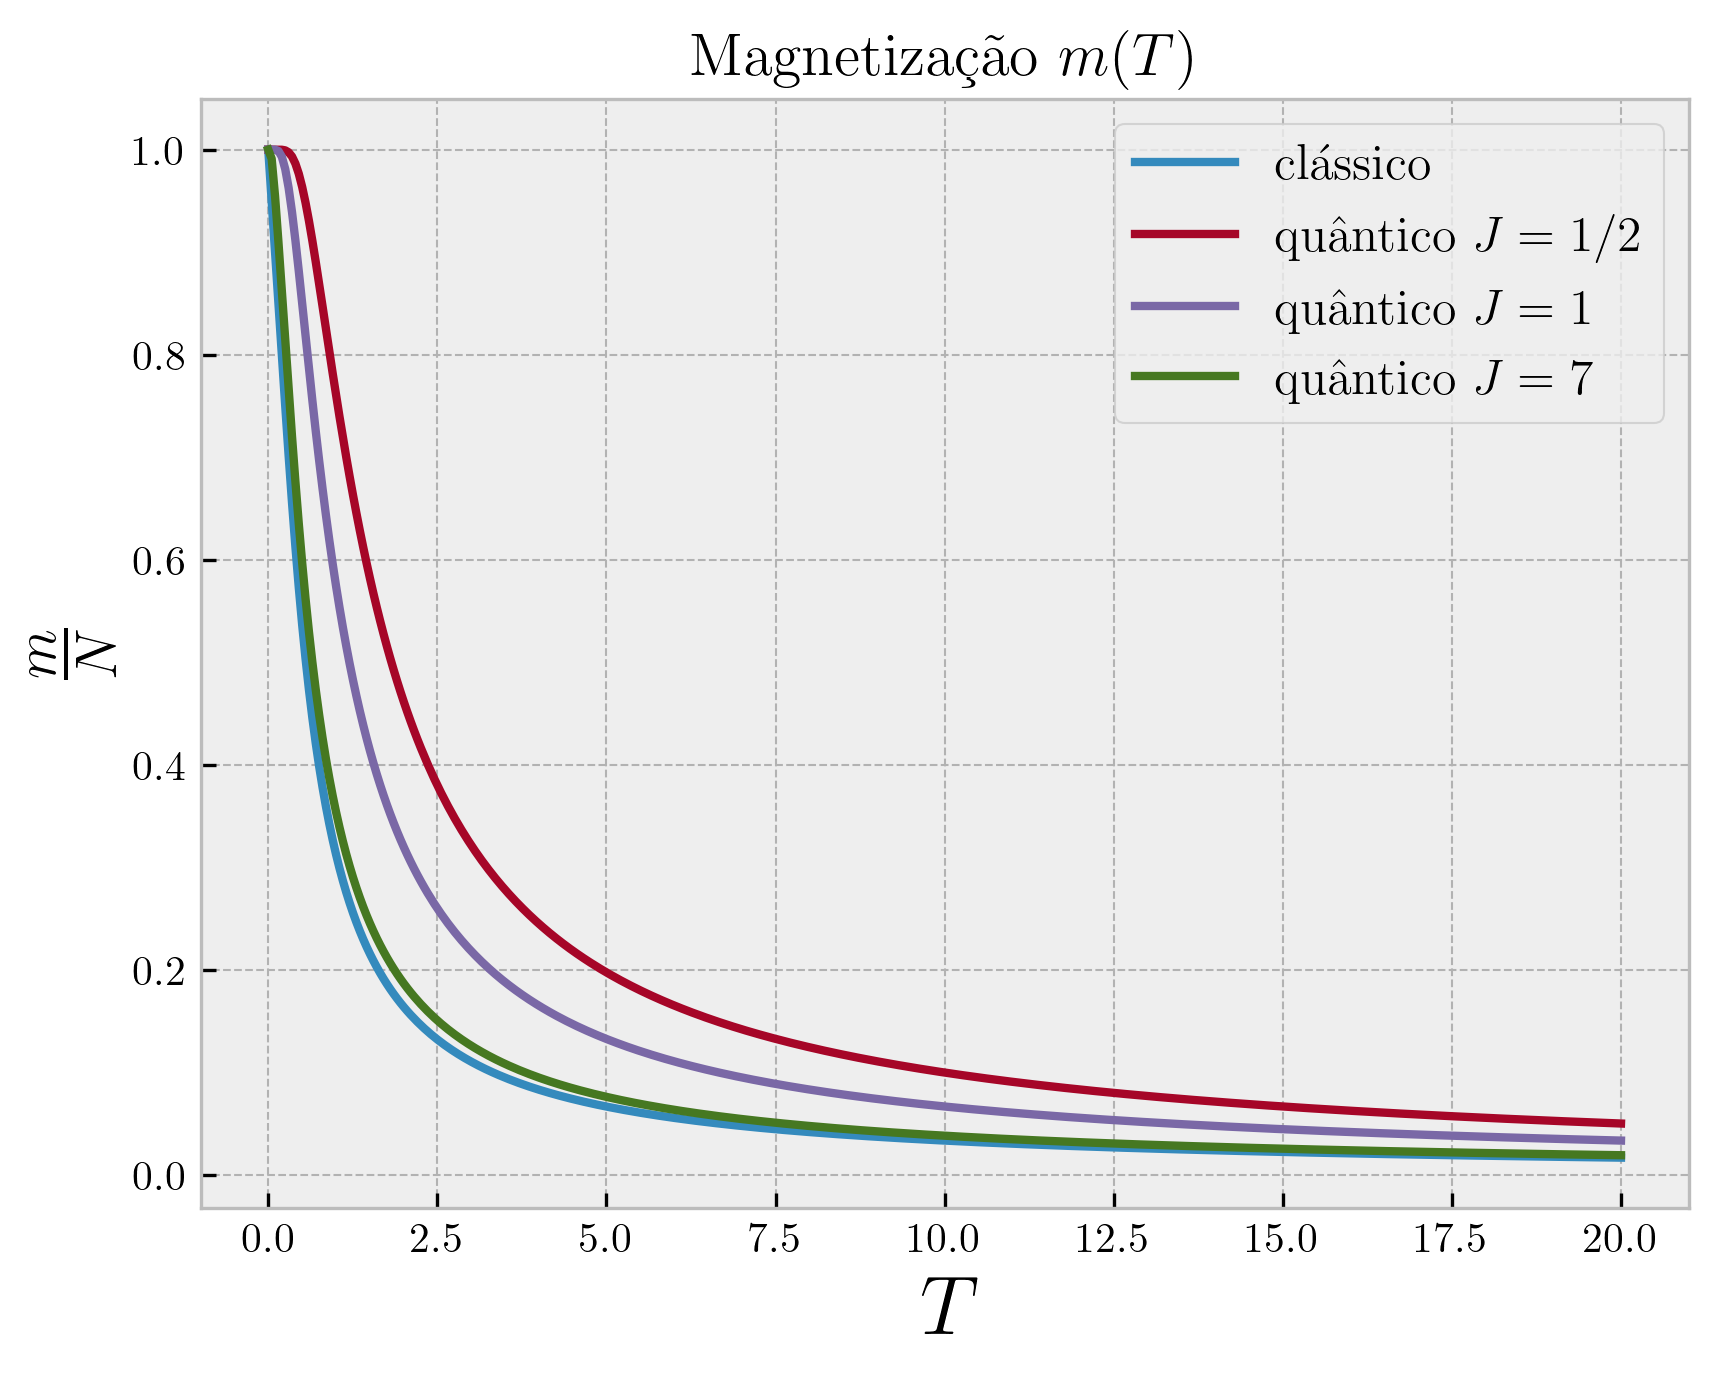
\includegraphics[width=0.7\linewidth]{fig/magnetiz.png}
\caption{Curva da magnetização $m(T)$. Foram usadas as unidades onde $\mu = B = k_B = 1$.}
\label{fig:magnetiz}
\end{figure}

Podemos ver na Figura \ref{fig:magnetiz} que em temperatura $T = 0$ a magnetização é total igual a 1, sendo alinhada com o campo magnético. Quando a temperatura aumenta as flutuações térmicas destroem a magnetização. Também vemos que a medida que o $J$ aumenta, a curva da magnetização quântica se aproxima da curva da magnetização clássica.

\n

A susceptibilidade magnética é dada por
$$
\chi = \pdvc{m}{B}{T,V,N} = N \mu^2 \beta L'(\beta \mu B),
$$
onde $L'(x) = 1/x^2 - \csch[2](x)$ é a derivada da função de Langevin.

\n\n

(b) A expansão da função de Langevin em torno de $x = 0$ no Mathematica nos dá $L(x) = \frac{x}{3} + O(x^2)$. Assim, para $T \to \infty$ ($\beta \to 0$), temos que a magnetização é
$$
m(T \to \infty) = \frac{N \mu^2 B}{3 k_B T} \implies \chi(T\to\infty) = \pdv{m(T\to\infty)}{B} = \frac{N\mu^2}{3 k_B T},
$$
que é justamente a lei de Curie $\chi \propto 1/T$, para $T \to \infty$.

\n

Agora faremos esse cálculo novamente, só que por meio da teoria de perturbação termodinâmica com $E_0 = 0$ e $V = -\sum_{i=1}^{N} \bm{\mu}_i \vdot \B = - \sum_{i=1}^{N} \mu B \cos(\theta_i)$. Essa teoria de perturbação se baseia na aproximação $e^{-\beta V(q,p)} \approx 1 - \beta V(q,p) + \frac{\beta^2 V(q,p)^2}{2}$, que vale somente para $\beta \to 0$, ou seja, no limite $T \to \infty$. Utilizando essa aproximação no cálculo da função de partição de uma partícula, temos
$$
Z_1' = \int e^{-\beta (E_0 + V(\theta,\vphi))} \dd{\Omega} = \int e^{-\beta V(\theta,\vphi)} \sin\theta \dd{\theta} \dd{\vphi} =
$$
$$
= \int_0^{2\pi} \dd{\vphi} \int_{-1}^{1} \qty[1 - \beta V(\theta,\vphi) + \frac{\beta^2}{2} V^2(\theta,\vphi)] \dd{(\cos\theta)} =
$$
$$
= 2\pi \int_{-1}^{1} \qty[1 + \beta \mu B \cos\theta + \frac{\beta^2\mu^2B^2}{2} \cos[2](\theta)] \dd{(\cos\theta)} =
$$
$$
= 2\pi \int_{-1}^{1} \qty[1 + \beta \mu B y + \frac{\beta^2\mu^2B^2}{2} y^2] \dd{y} =
$$
$$
= 4\pi \qty[1 + \frac{(\beta\mu B)^2}{6}].
$$

Usando que $\log(1+x) \approx x$, temos que $\log Z_1' \approx \log(4\pi) + \frac{(\beta\mu B)^2}{6}$. Lembrando que $F = -\frac{N}{\beta} \log Z_1' + \frac{1}{\beta} \log N!$, temos
$$
m = -\pdvc{F}{B}{T,V,N} = \frac{N}{\beta} \pdv{\log Z_1'}{B} = \frac{N}{\beta} \cdot \frac{\beta^2\mu^2 B}{3} =
\frac{N\mu^2 B}{3 k_B T}.
$$

A susceptibilidade é então
$$
\chi = \pdvc{m}{B}{T,V,N} = \frac{N\mu^2}{3 k_B T},
$$
que é justamente o resultado que obtemos para $\chi(T \to \infty)$, só que dessa vez utilizamos a teoria de perturbação termodinâmica para obter a lei de Curie.

\n\n

Para o caso quântico, temos que $V = - \sum_{i=1}^{N} \hat{\mu}_i^z B$, onde $\hat{\mu}_i = \mu \sigma_i^z$ é um operador e $\sigma^z$ é a matriz de Pauli. Nesse caso, podemos utilizar diretamente a fórmula vista em aula para a perturbação termodinâmica
$$
F = F_0 + \ev{V}_0 - \frac{\beta}{2} \ev{(V-\ev{V}_0)^2}_0.
$$

No caso, temos que $F_0$ não depende de $B$ e portanto não contribui para magnetização ou susceptibilidade. O primeiro termo é
$$
\ev{V}_0 = -\mu B \sum_{i=1}^{N} \ev{\sigma_i^z}_0,
$$
mas o valor esperado $\ev{\sigma_i^z}_0$ é nulo pois os autovalores da matriz de Pauli são $+1$ e $-1$. Para o segundo termo, temos que
$$
\ev{(V-\ev{V}_0)^2}_0 = \ev{V^2}_0 = \mu^2 B^2 \ev{\qty(\sum_{i=1}^N \sigma_i^z)^2}_0 = \mu^2 B^2 \sum_{i=1}^N \ev{(\sigma_i^z)^2}_0 = N \mu^2 B^2,
$$
onde os termos $\ev{\s_i^z \s_j^z}_0 = 0$ pois as duas matrizes de Pauli são de partículas diferentes e não-interagentes, portanto independentes, e também usei que $(\s_i^z)^2 = 1$. Com isso temos que
$$
F = F_0 - \frac{N \mu^2 B^2}{2 k_B T} \implies \chi = -\qty(\pdv[2]{F}{B})_{T,V,N} = \frac{N\mu^2}{k_B T},
$$
que é quase o mesmo resultado do caso clássico a menos de um fator $3$, que não sei explicar...



\end{document}
